\chapter{Methods}
\label{chap:methods}
\TODO{Intro - of chapter and probably other chapter name}\\
To train any kind of statistical or machine learning model we need a large enough dataset. For our initial studies we will use various subsets of the QM9 dataset \parencite{ref:article1_qm9, ref:article2_qm9}. \TODO{More intro \& reference to Background chapter}

\section{QM9 dataset \parencite{ref:data_qm9}}
\label{sec:qm9}
Time savings given through faster convergence are especially relevant for larger systems where the number of SCF iterations are and especially the number of integrals to be calculated are large. Stated differently, it is of little interest to optimize guessing methods for small systems which converge in a near instantly on conventional hardware. Furthermore, a constant input and output size is required to train most machine learning models. \\
The QM9 dataset \parencite{ref:article1_qm9,ref:article2_qm9} ticks both of these two boxes. It offers a diverse variety of molecules from as little as 3 constituent atoms up to 29 atoms. Additionally, there are large enough chunks of constitutional isomers to train models on these subsets of same sized matrices. The distribution of molecules by atom count with the predominant constitutional isomers is shown in \autoref{fig:method_qm9_overview}.
\begin{figure}[H]
    \centering
    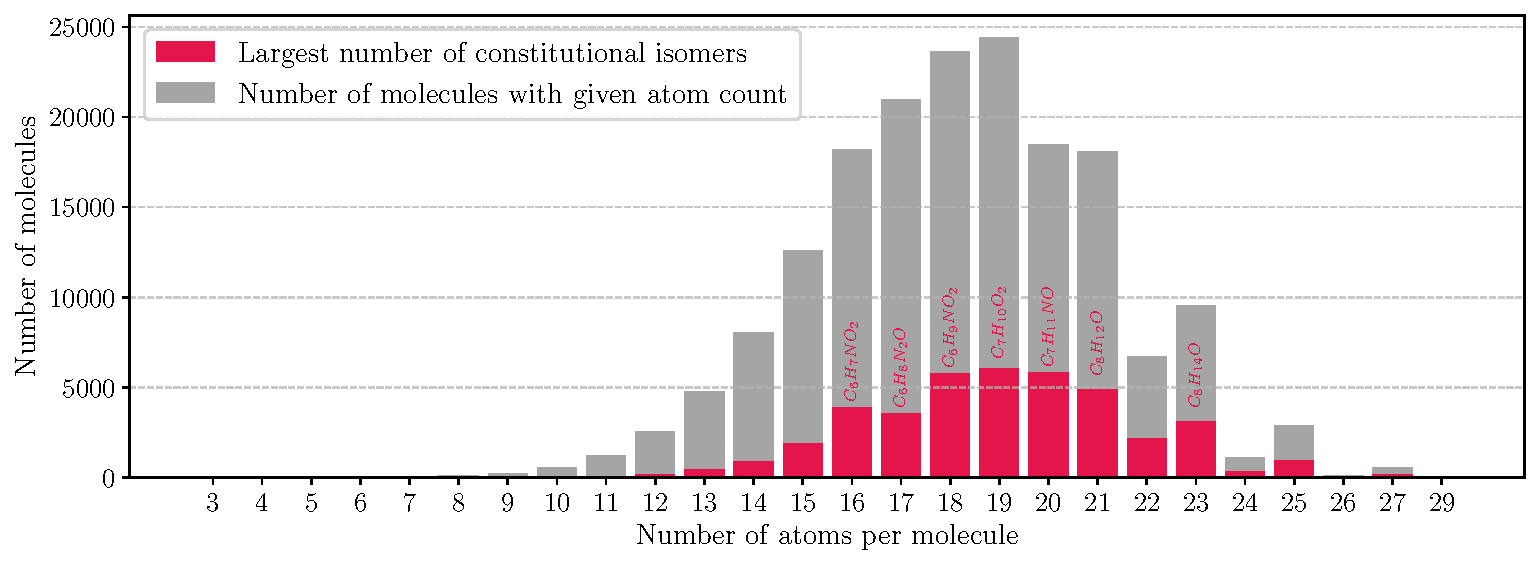
\includegraphics[width=\textwidth]{../fig/qm9_general/qm9_overview_stacked_bar.pdf}
    \caption[QM9 dataset overview]{Overview of the QM9 dataset. The dataset contains 134k molecules with up to nine heavy - \ch{C} \ch{O} \ch{N} \ch{F} - atoms. Large groups of constitutional isomers are present (largest depicted in red). The properties are calculated using DFT with the B3LYP functional and the 6-31G(2df,p) basis set.}
    \label{fig:method_qm9_overview}
\end{figure}


\section{Fock Matrix prediction: A first trial}
\label{sec:first_predictions}
SCF methods by nature initially need a density matrix to start off their iterative calculations. Independent of the way the initial guess is chosen the computational effort of this step should be negligible compared to the actual SCF iterations. 
\TODO{Add more details about the Fock matrix prediction - Reasoning for the choice.}

As explained in \autoref{sec:background} (\TODO{Background SCF}) the density matrix $P$ is calculated from the coefficient matrix $C$ which is obtained from the eigenvalue problem of the Fock matrix $F$:
\begin{equation}
    FC = SC\varepsilon \rightarrow P = 2CC^T
\end{equation}
Effectively, one performs part of the SCF cycle here to obtain the density matrix, which ideally should be close to the final density matrix. This step takes $\bigO{N^3}$ time, which is assymtotically faster than the $\bigO{N^4}$ time of the SCF cycle. 

The schematic workflow of generating a density matrix from the overlap matrix is shown in \autoref{fig:method_data_flow}. While the overlap and density might look very similar and one might think that predicting the density matrix directly from the overlap matrix would be easier. However, learning the Fock matrix tends to involve fewer strict physical constraints. A Fock matrix primarily needs to be Hermitian, while a density matrix must be strictly positive semidefinite by construction, as well as normalized to the correct number of electrons. That makes direct density matrix learning more challenging, whereas learning the Fock matrix and then obtaining the density through the diagonalization could yield better results. \TODO{Reference?}
\noindent
\begin{figure}
    \centering
    \begin{tikzpicture}[scale=1, every node/.style={transform shape}]

        % Skalierungsfaktor für drei Bilder + Zwischenraum
        \def\imgwidth{0.30\linewidth}

        % Erstes Bild mit Titel
        \node[anchor=south west, inner sep=0] (img1) at (0,0)
            {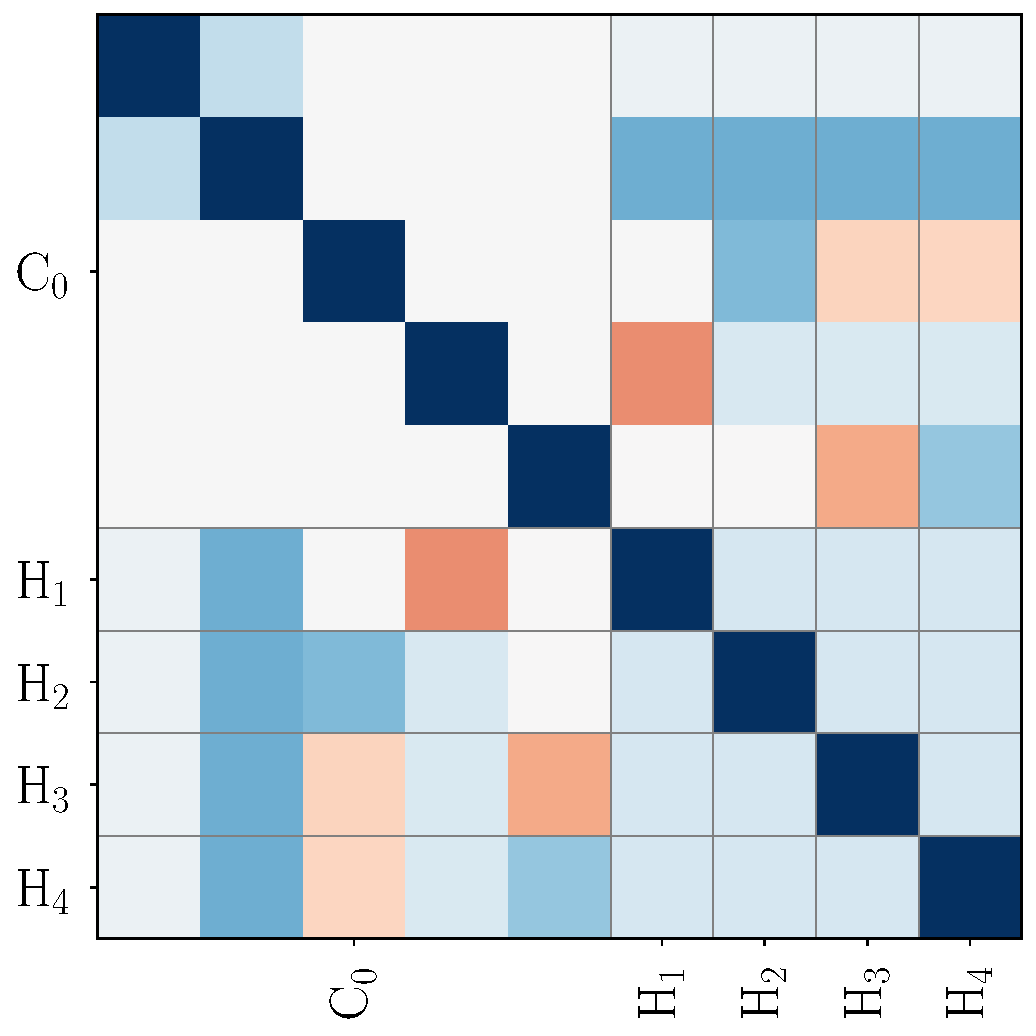
\includegraphics[width=\imgwidth]{../fig/c5h4n2o2/overlap_dsgdb9nsd_000001.pdf}};
        \node[above=2pt of img1.north, anchor=south, font=\small, xshift=10pt] {Overlap};

        % Zweites Bild mit Titel
        \node[anchor=south west, inner sep=0] (img2) at (5.1,0)
            {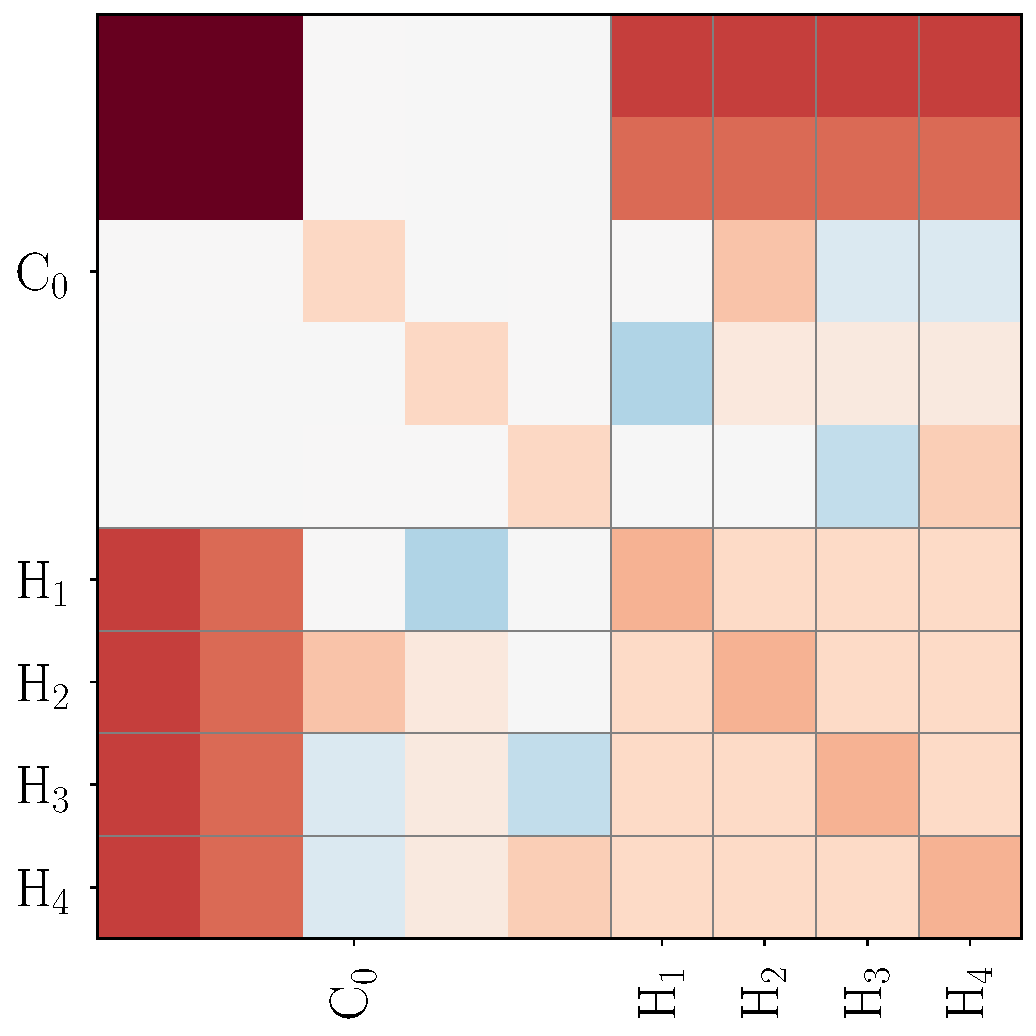
\includegraphics[width=\imgwidth]{../fig/c5h4n2o2/fock_dsgdb9nsd_000001.pdf}};
        \node[above=2pt of img2.north, anchor=south, font=\small, xshift=10pt] {Fock};

        % Drittes Bild mit Titel
        \node[anchor=south west, inner sep=0] (img3) at (10.2,0)
            {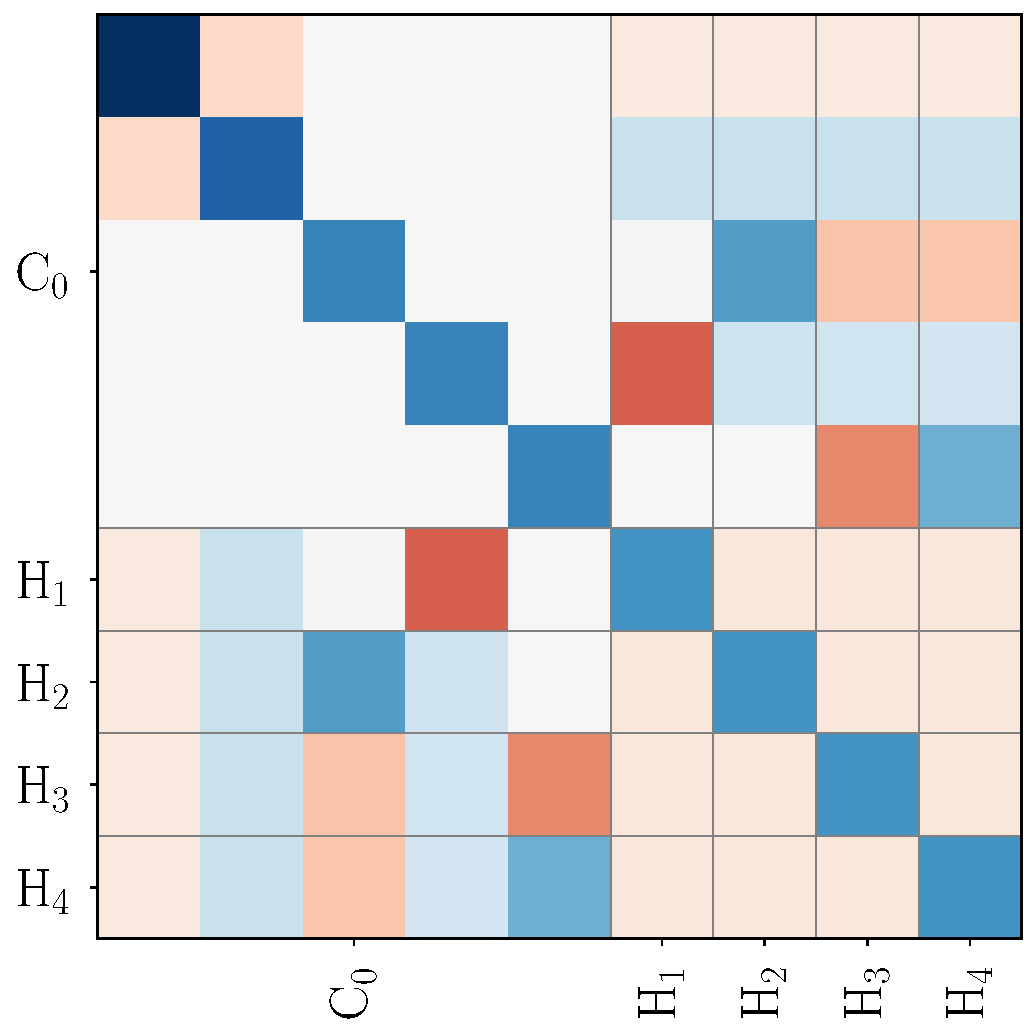
\includegraphics[width=\imgwidth]{../fig/c5h4n2o2/density_dsgdb9nsd_000001.pdf}};
        \node[above=2pt of img3.north, anchor=south, font=\small, xshift=10pt] {Density};
        
        % Pfeil 1: ML model
        \draw[->, thick] (4.7,2.4) -- node[above, align=center, font=\tiny]{ML\\model} (5.2,2.4);

        \draw[->, thick] (9.8,2.4) -- node[above, font=\tiny, yshift=1pt]{$P{=}2CC^{\mathrm{T}}$} (10.3,2.4);
    \end{tikzpicture}
    \caption[Schematic overview data flow]{Schematic overview of the data flow (using \ch{CH4}): overlap matrix to Fock matrix via ML model prediction, and construction of the density matrix from the Fock matrix.}
    \label{fig:method_data_flow}
\end{figure}

\subsection{\ch{C5H4N2O2}}
\label{subsec:qm9_c5h4n2o2}
As a proof of concept we will use 508 constitutional isomers\footnote{From the 509 constitutional isomers of \ch{C5H4N2O2} only 508 converged using the sto-3g basis and the B3LYP functional.} of \ch{C5H4N2O2} from the QM9 dataset. 
Single point RKS simulations in \textsc{PySCF} \parencite{ref:pyscf} were performed for these molecules using the B3LYP\footnote{B3LYPG was used to be consitant with the Gaussian} functional and the sto-3g basis. The resulting converged density-, fock-, and overlap-matrices were saved for future training purposes. For our very minimal basis these matrices are of size $49 \times 49$ as can be seen for a converged density in \autoref{fig:density_dsgdb9nsd_022700}. 
Due to the symmetry of the matrices we can discard nearly half of the elements and are left with 1225 features to learn. A rule of thumb for training classical statistical models is to have at least 10 samples per feature. \parencite{ref:rule_of_10} The given dataset of 508 samples is therefore far off from this rule. Keeping this in mind, we will start off our endevaour with a Ridge regression model as a first trial. 

\begin{figure}
    \centering
    \includegraphics[width=\textwidth]{../fig/c5h4n2o2/density\_dsgdb9nsd\_022700.pdf}
    \caption[Density matrix of dsgdb9nsd\_022700 in the sto-3g basis with theory level B3LYP]{Converged density of dsgdb9nsd\_022700 in the sto-3g basis with theory level B3LYP. The density matrix is of size $49 \times 49$ and is symmetric. The diagonal elements are the occupation numbers of the corresponding orbitals.}
    \label{fig:density_dsgdb9nsd_022700}
\end{figure}

\textbf{Ridge regression model}\\
The Ridge regression is setup with a typical $80 / 20$ train/test split. Overlap (input) as well as Fock (output) matrices are flattend and used as is (rescaling did not improve model accuracy). Using a 5-fold cross validation the model is a Multi-Ouput-Regressor is trained using \textsc{scikit-learn} \parencite{ref:sk-learn} with equally $\log_{10}$-spaced $L^2$-regularization parameter $\alpha$ values ranging from $10^{-2}$ to $10^{3}$. Subsequently, the model is retrained with the arithmetic mean of the best performing $\alpha$ values. For the Fock matrix prediction the model yields a RMSE of $0.046$ on the training set and $0.059$ on the test set which indicates slight overfitting. Using the F-Score metric \parencite{ref:Lehtola2019} (outlined in \autoref{subsec:background_cost_function}) which can be used as a proxy for the convergence speed we obtain mixed results. 

\begin{table}[h]
    \centering
    \caption{Comparison of Mean F-score on Test Set}
    \label{tab:fscore_comparison}
    \begin{tabular}{l
                    S[table-format=1.2(2)]
                    S[table-format=1.3(3)]
                    S[table-format=1.2(2)]
                    S[table-format=1.3(3)]
                    S[table-format=1.3(3)]
                    S[table-format=1.3(3)]}
        \toprule
        \textbf{Method} & \texttt{Ridge-model} & \texttt{minao} & \texttt{1e} & \texttt{atom} & \texttt{huckel} & \texttt{vsap} \\
        \midrule
        F-score / 1 & 0.88 \pm 0.06 & 0.899 \pm 0.002 & 0.71 \pm 0.02 & 0.802 \pm 0.001 & 0.840 \pm 0.010 & 0.993 \pm 0.002 \\
        Iterations / 1 & & & & & & \\
        Not-Converged / \% & & & & & & \\
        \bottomrule
    \end{tabular}
\end{table}


\TODO{Rescaling hat es schlechter gemacht in unserem Fall.}
\section{Software and Implementation Specifics}
\label{sec:software_and_implementation}
Reproducability crisis
\section{Cost function}
\section{Dataset}